\documentclass[french]{nakrule}

\usepackage{infoBulle}
\usepackage{yFlatTable}
\usepackage{multirow}
\usepackage{calc}

\author{Samuel Riedo \& Pascal Roulin}
\title{Space Invaders}
\subtitle{Projet intégré - Système numérique}

\makeatletter
\let\runauthor\@author
\let\runtitle\@title
\makeatother

%\definecolor{mainColor}{RGB}{255,50,50}
\definecolor{blockColor}{RGB}{255,160,160}

\begin{document}


\titleTwo[pictures/title]

%--------------------------------------------------------------------
\chapter{Introduction}
\label{introduction}
%--------------------------------------------------------------------

\emph{Space Invaders} est un jeu vidéo d'arcade créé par Tomohiro Nishikado, paru pour
la première fois en 1978 au Japon. Il est l'un des tout premier \emph{Shoot 'em
  up}, c'est-à-dire un type de jeux consistant à abatre un grand nombre d'ennemies en
leur tirant dessus. Le principe du jeu consiste en un vasseau spacial attaqué
par des vagues d'aliens qu'il doit détruire en leur tirant dessus sans se faire
toucher par les tirs des aliens.

\emph{Space Invaders} connu rapidement un succès mondial et est aujourd'hui
considéré comme un grand classique de l'univers vidéoludique. Il a de ce fait
connu de nombreux ports et suites sur un grand nombre de plate-forme, vieille
comme récente.

\section{Super Mario Bros}
\label{sec:mario}

Dans un premier temps, nous avions souhaité reproduire \emph{Super Mario Bros}.
La première tentative pour recréer le monde 1-1 du jeu original fut de créer
toute la map en une image, puis de la stocker dans une RAM ou ROM.
Un scalling de 4 permet de drastiquement réduire le nombre de pixels à stocker,
en passant de 6400x800 pour l'image d'origine à 1600x150 pour celle que nous
utiliserons.
Ceci représentait \si{240.000} pixels à stocker. En prenant en compte qu'un pixel
fait exactement un Byte (deux bits pour la composante bleu, trois pour la rouge
et trois pour la verte), les RAM et ROM à disposition de la Spartan 6
XC6LX16-CS324 ne pouvaient pas stocker toutes ses données.

Afin de contourner ce problème, l'image de base a été diviser en 8 images plus
petites, faisant chacune 200x150 pixels, soit 30kB. Il était alors possible de
stocker une image dans une ROM/RAM, puis une deuxième dans une seconde ROM/RAM,
mais il était à nouveau impossible d'enregistrer les six suivantes sans dépasser
les capacités de la carte.

Devant ses limitations hardware, la décision fu prise de changer de jeu. Il nous
est apparu qu'avoir un font statique, ou alors une répétition permannente d'un
même arrière plan était indispensable pour que le projet soit synthétisable sur
notre carte. Un jeu tel que \emph{Super Mario Bros}, avec des mondes très
différents et non répétifs, n'est pas adapté à la programmation VHDL sur un
hardware limité.


\clearpage
\symmetricalPage

\section{Gameplay}
\label{sec:gameplay}

Space Invaders est un jeu en deux dimension, aussi appelé jeu en 2D ou tout
simplement jeu 2D. Le joueur contrôle un vaisseau spatial pouvant se déplacer
uniquement sur l'axe $X$, et tirer des laser vers le haut de l'écran. Il est
confronté à plusieurs aliens, se déplaçant aléatoirement dans la partie
supérieur de l'écran. Ces derniers tire aléatoirement des lasers vers le bat
pour détruire le vaisseau spacial contrôlé par le joueur.

Si le vaisseau du joueur se fait toucher par un laser alien, la partie est
perdue. Si, au contraire, le joueur réussit à détruire tous les aliens sans se
faire lui-même toucher, il gagne la partie. La figure ci-dessus représente une
partie typique de \emph{Space Invaders} sur borne arcade tel que le jeu était
lors de son lancement initial en 1978.

\begin{figure}[ht]
  \centering
  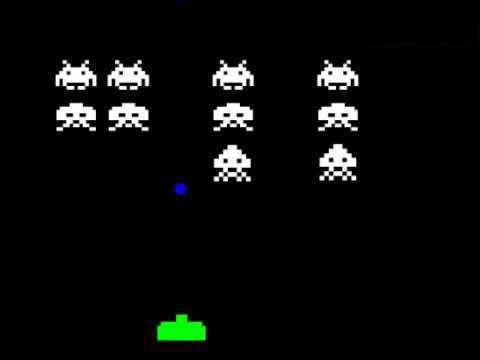
\includegraphics[width=.6\textwidth]{pictures/gameOnArcade}
  \caption{Space Invaders sur borne arcade}
  \label{gameOnArcade}
\end{figure}

Le vaisseau du joueur est représenté par la forme verte. Ce dernier à tiré un
laser, symbolisé par un poinds bleu. Les aliens, au nombre de 10, ont déjà été
partiellement déssimer. Au début d'une partie, leur nombre et leur disposition
forme une grille rectangulaire complète.

\infoInfo{Types d'aliens}{Bien que les aliens peuvent avoir plusieurs formes
  différents (trois sur la figure \ref{gameOnArcade}), celà n'influence en rien
  leur comportement. Il ne s'agit ni plus ni moins que d'un skin.}

Les version suivantes de space invaders implémenteront de nouvelles
fonctionnalités, tel que:\vspace{.1in}
\begin{items}
\item Score, déterminer par les aliens détruits et le temps pour y arriver.
\item Vaisseau alien traversant l'écran horizontalement de façon aléatoire. Le
  détruire rapport des points bonus.
\item Bouclier pour protéger le vaisseaux.
\end{items}




% --------------------------------------------------------------------
\asymmetricalPage
\chapter{Architecture}
\label{architecture}

La réalisation du projet fut divisé en 6 principaux blocs, plus un top module et
un package. Trois de ces blocs furent repris du travail pratique concernant
l'affichage par VGA, alors que les autres ont été spécialement implémentés pour
ce projet.

Le fait d'avoir déjà une base de départ nous a poussé à implémentés le jeu
fonction par fonction, puis de tester et debugguer chaque nouvel ajout dès qu'il
fut coder. Cette approche présente l'avantage, contrairement à un developpement
de chaque composants indépendamment les uns des autres, de réduire le risque
d'incompatibilité entre deux composants à fin ainsi que le lourd travaille de
debuggage final. En revanche, cette technique ne permet pas de répartir
efficassement le travail dans une équipe constituée de nombreuse personnes.

Bien que nous puissons tester le bon fonctionnement de chaque blocs et fonctions
directement en programmant la FPGA pour voir le résultat sur l'écran, chaque
bloc sera testé par une macro pour valider tous les cas pouvant intervenir dans
le déroulement d'une partie. De plus, deux composants, \emph{Input} et
\emph{rocketManager}, seront testé via un testbench.

\symmetricalPage

\section{alienRocket}
\label{sec:label}


\begin{wrapfigure}[23]{r}{.55\textwidth}
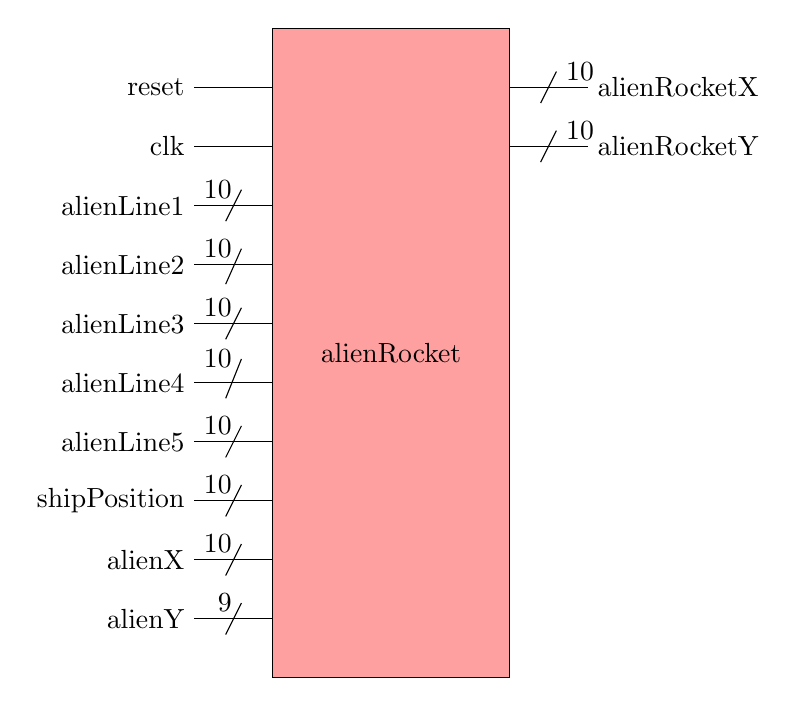
\begin{tikzpicture}
  \draw[fill=blockColor] (0,0) rectangle node{alienRocket}(3,-8.25);
  % Inputs
  \draw (-1,-.75) node[left]{reset}-- (0,-.75);
  \draw (-1,-1.5) node[left]{clk}-- (0,-1.5);
  \draw (-1,-2.25) node[left]{alienLine1}-- (0,-2.25);
  \draw (-.4,-2.05) node[left]{10} -- (-.6, -2.45);
  \draw (-1,-3) node[left]{alienLine2}-- (0,-3);
  \draw (-.4,-2.8) node[left]{10} -- (-.6, -3.25);
  \draw (-1,-3.75) node[left]{alienLine3}-- (0,-3.75);
  \draw (-.4,-3.55) node[left]{10} -- (-.6, -3.95);
  \draw (-1,-4.5) node[left]{alienLine4}-- (0,-4.5);
  \draw (-.4,-4.2) node[left]{10} -- (-.6, -4.7);
  \draw (-1,-5.25) node[left]{alienLine5}-- (0,-5.25);
  \draw (-.4,-5.05) node[left]{10} -- (-.6, -5.45);
  \draw (-1,-6) node[left]{shipPosition}-- (0,-6);
  \draw (-.4,-5.8) node[left]{10} -- (-.6, -6.2);
  \draw (-1,-6.75) node[left]{alienX}-- (0,-6.75);
  \draw (-.4,-6.55) node[left]{10} -- (-.6, -6.95);
  \draw (-1,-7.5) node[left]{alienY}-- (0,-7.5);
  \draw (-.4,-7.3) node[left]{9} -- (-.6, -7.7);
  % Outputs
  \draw (4,-.75) node[right]{alienRocketX}-- (3,-.75);
  \draw (3.6,-.55) node[right]{10} -- (3.4, -.95);
  \draw (4,-1.5) node[right]{alienRocketY}-- (3,-1.5);
  \draw (3.6,-1.3) node[right]{10} -- (3.4, -1.7);
\end{tikzpicture}
\caption{Schéma bloc}
\label{alienRocketBloc}
\end{wrapfigure}

Le bloc \emph{alienRocket} gère les roquettes, aussi appelé laser ou missile, tirés par
les aliens en direction du spationef. Il est chargé de générer de nouveaux
missiles ainsi que de transmettre les informatins nécessaire au bloc \emph{Display} pour afficher
correctement une roquette à l'écran.
Dans notre implémentation du jeu, le joueur fait face à 50 aliens, réparties en
une grille de 5 lignes et 10 colonnes (tableau \ref{alientable}). Par colonne,
chaque aliens le plus proche du bat de l'écran peut tirer une roquette vers le
bat pour tenter de détruire le vaisseau du joueur. Une seule roquette peut être
affiché à l'écran en même temps (sans compter les tirs du joueur). Cela signifie
que tant que le missile n'a pas atteint le bat de l'écran, les aliens ne peuvent
pas en tirer un nouveau.

Lorsqu'une roquette peut être tiré, le choix de la colonne d'alien pouvant tirer
se fait de manière aléatoire entre toutes les colonnes qui contiennes au moi un
alien. Par exemple, soit les aliens encore en vie selon le tableau
\ref{alientable}. Une roquette peut être tiré depuis les aliens 0-4 et 7-9 de la
ligne 5 (alienLine5), ainsi que depuis les alien 5 et 6 de la ligne 4 (alienLine4).

\begin{table}[ht]
  \centering
  \begin{tabular}{c c c c c c c c c c c}
    & \multicolumn{10}{c}{Index}\\
    & 0 & 1 & 2 & 3 & 4 & 5 & 6 & 7 & 8 & 9 \\
    $\begin{matrix}\text{alienLine1}\\ \text{ }\end{matrix}$ & 
\includegraphics[width=.05\textwidth]{pictures/aliens/blue}&
    
\includegraphics[width=.05\textwidth]{pictures/aliens/blue}&
    
\includegraphics[width=.05\textwidth]{pictures/aliens/blue}&
    
\includegraphics[width=.05\textwidth]{pictures/aliens/blue}&
    
\includegraphics[width=.05\textwidth]{pictures/aliens/blue}&
    
\includegraphics[width=.05\textwidth]{pictures/aliens/blue}&
    
\includegraphics[width=.05\textwidth]{pictures/aliens/blue}&
    
\includegraphics[width=.05\textwidth]{pictures/aliens/blue}&
    
\includegraphics[width=.05\textwidth]{pictures/aliens/blue}&
    
\includegraphics[width=.05\textwidth]{pictures/aliens/blue}\\
    $\begin{matrix}\text{alienLine2}\\ \text{ }\end{matrix}$ & 
\includegraphics[width=.05\textwidth]{pictures/aliens/DarkBlue}&
    
\includegraphics[width=.05\textwidth]{pictures/aliens/DarkBlue}&
    
\includegraphics[width=.05\textwidth]{pictures/aliens/DarkBlue}&
    
\includegraphics[width=.05\textwidth]{pictures/aliens/DarkBlue}&
    
\includegraphics[width=.05\textwidth]{pictures/aliens/DarkBlue}&
    
\includegraphics[width=.05\textwidth]{pictures/aliens/DarkBlue}&
    
\includegraphics[width=.05\textwidth]{pictures/aliens/DarkBlue}&
    
\includegraphics[width=.05\textwidth]{pictures/aliens/DarkBlue}&
    
\includegraphics[width=.05\textwidth]{pictures/aliens/DarkBlue}&
    
\includegraphics[width=.05\textwidth]{pictures/aliens/DarkBlue}\\
    $\begin{matrix}\text{alienLine3}\\ \text{ }\end{matrix}$ & 
\includegraphics[width=.05\textwidth]{pictures/aliens/green}&
    
\includegraphics[width=.05\textwidth]{pictures/aliens/green}&
    
\includegraphics[width=.05\textwidth]{pictures/aliens/green}&
    
\includegraphics[width=.05\textwidth]{pictures/aliens/green}&
    
\includegraphics[width=.05\textwidth]{pictures/aliens/green}&
    
\includegraphics[width=.05\textwidth]{pictures/aliens/green}&
    
\includegraphics[width=.05\textwidth]{pictures/aliens/green}&
    
\includegraphics[width=.05\textwidth]{pictures/aliens/green}&
    
\includegraphics[width=.05\textwidth]{pictures/aliens/green}&
    
\includegraphics[width=.05\textwidth]{pictures/aliens/green}\\
    $\begin{matrix}\text{alienLine4}\\ \text{ }\end{matrix}$ & 
\includegraphics[width=.05\textwidth]{pictures/aliens/purple}&
    
\includegraphics[width=.05\textwidth]{pictures/aliens/purple}&
    
\includegraphics[width=.05\textwidth]{pictures/aliens/purple}&
    
\includegraphics[width=.05\textwidth]{pictures/aliens/purple}&
    
\includegraphics[width=.05\textwidth]{pictures/aliens/purple}&
    
\includegraphics[width=.05\textwidth]{pictures/aliens/purple}&
    
\includegraphics[width=.05\textwidth]{pictures/aliens/purple}&
    
\includegraphics[width=.05\textwidth]{pictures/aliens/purple}&
    
\includegraphics[width=.05\textwidth]{pictures/aliens/purple}&
    
\includegraphics[width=.05\textwidth]{pictures/aliens/purple}\\
    $\begin{matrix}\text{alienLine5}\\ \text{ }\end{matrix}$ & 
\includegraphics[width=.05\textwidth]{pictures/aliens/yellow}&
    
\includegraphics[width=.05\textwidth]{pictures/aliens/yellow}&
    
\includegraphics[width=.05\textwidth]{pictures/aliens/yellow}&
    
\includegraphics[width=.05\textwidth]{pictures/aliens/yellow}&
    
\includegraphics[width=.05\textwidth]{pictures/aliens/yellow}&&&
    
\includegraphics[width=.05\textwidth]{pictures/aliens/yellow}&
    
\includegraphics[width=.05\textwidth]{pictures/aliens/yellow}&
    
\includegraphics[width=.05\textwidth]{pictures/aliens/yellow}\\
  \end{tabular}
  \caption{Gestion des aliens dans le jeux}
  \label{alientable}
\end{table}


\clearpage

\subsection{Entrées \& Sorties}
\label{subsec:Entrées_Sorties_alienRocket}

\begin{descr}
  \itemColor{reset} Reset du circuit, actif à l'état haut.
  \itemColor{clk} Horloge 40MHz, active sur front montant.
  \itemColor{alienLine1} Indique, par un 0 un alien vivant, et par 1 un alien
  mort dans la ligne d'alien de la partie supérieur de l'écran.
  \itemColor{alienLine2} Identique à alienLine1, pour la ligne d'alien en dessous.
  \itemColor{alienLine3} Identique à alienLine2, pour la ligne d'alien en dessous.
  \itemColor{alienLine4} Identique à alienLine3, pour la ligne d'alien en dessous.
  \itemColor{alienLine5} Identique à alienLine4, pour la ligne d'alien en dessous.
  \itemColor{shipPosition} Nombre de pixels entre le bord gauche de l'écran et
  le bord droit du vaisseau de joueur. Cette valeur est utilisé pour générer de l'aléatoire.
  \itemColor{alienX} Nombre de pixels entre le bord gauche de l'écran et le
  board droit des aliens à l'index 0.
  \itemColor{alienY} Nombre de pixels entre le haut de l'écran et le bord
  supérieur des aliens contenues dans \emph{alienLine1}.
  \itemColor{alienRocketX} Nombre de pixels entre le bord gauche de l'écran et
  la rocket tirée par les aliens.
  \itemColor{alienRocketY} Nombre de pixels entre le le haut de l'écran et le
  haut de la rocket tirée par les aliens.
\end{descr}

\clearpage

\section{Digital Clock Management}
\label{sec:dcm}

\begin{wrapfigure}[10]{r}{.5\textwidth}
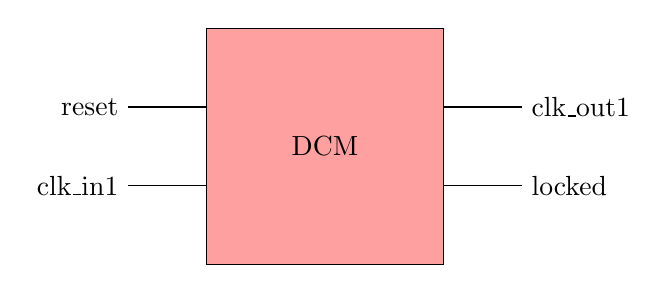
\begin{tikzpicture}
  \draw[fill=blockColor] (0,0) rectangle node{DCM}(3,3);
  \draw (-1,1) node[left]{clk\_in1}-- (0,1);
  \draw (-1,2) node[left]{reset}-- (0,2);
  \draw (4,2) node[right]{clk\_out1}-- (3,2);
  \draw (4,1) node[right]{locked}-- (3,1);
\end{tikzpicture}
\caption{Schéma bloc}
\label{dcmBloc}
\end{wrapfigure}

La norme VGA utilise une fréquence de 40MHz pour le balayage de l’écran. Or,
l’horloge intégrée à notre carte dispose d’une fréquence de 100MHz. Le bloc DCM
crée une horloge de 40MHz grâce à une horloge d'entrée de 100MHz.
Ce type de montage étant très courant, il existe des outils, appelé IP Core, pour générer un
composant selon nos besoins.

\subsection{Entrées \& Sorties}
\label{subsec:Entrées_Sorties_dmc}

\begin{descr}
  \itemColor{reset} Reset du circuit, actif à l'état haut.
  \itemColor{clk\_in1} Horloge 100MHz, active sur front montant.
  \itemColor{clk\_out1} Horloge 40MHz.
  \itemColor{locked} Sortie non utilisée.
\end{descr}

\clearpage

\section{Display}
\label{sec:display}

\begin{wrapfigure}{r}{.6\textwidth}
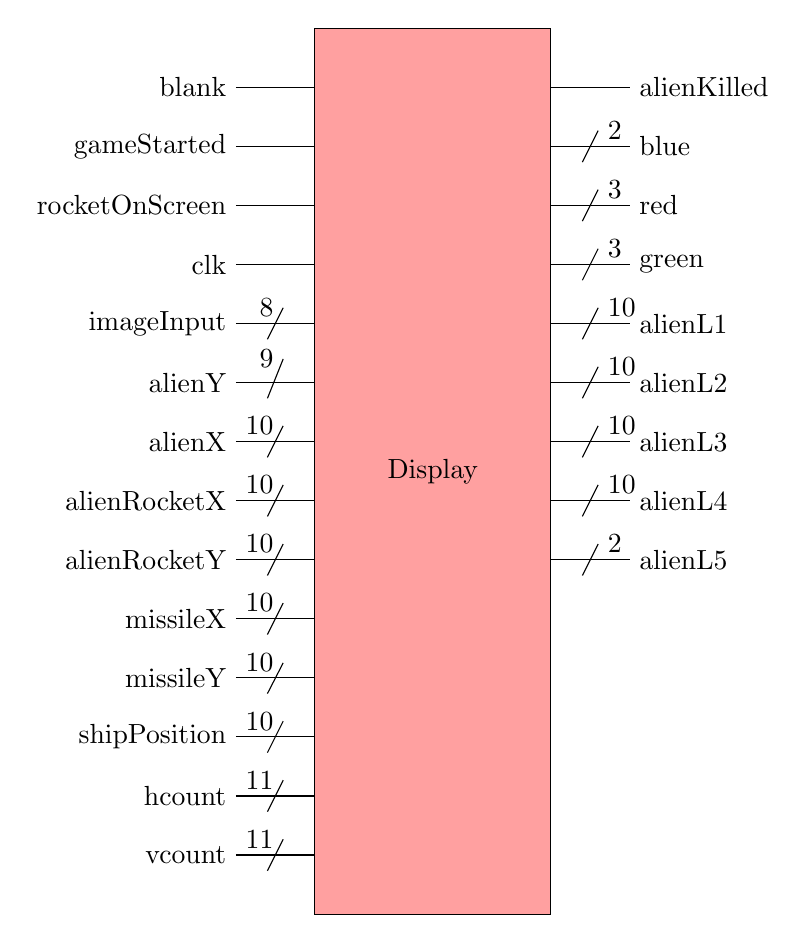
\begin{tikzpicture}
  \draw[fill=blockColor] (0,0) rectangle node{Display}(3,-11.25);
  % Inputs
  \draw (-1,-.75) node[left]{blank}-- (0,-.75);
  \draw (-1,-1.5) node[left]{gameStarted}-- (0,-1.5);
  \draw (-1,-2.25) node[left]{rocketOnScreen}-- (0,-2.25);
  \draw (-1,-3) node[left]{clk}-- (0,-3);
  \draw (-1,-3.75) node[left]{imageInput}-- (0,-3.75);
  \draw (-.4,-3.55) node[left]{8} -- (-.6, -3.95);
  \draw (-1,-4.5) node[left]{alienY}-- (0,-4.5);
  \draw (-.4,-4.2) node[left]{9} -- (-.6, -4.7);
  \draw (-1,-5.25) node[left]{alienX}-- (0,-5.25);
  \draw (-.4,-5.05) node[left]{10} -- (-.6, -5.45);
  \draw (-1,-6) node[left]{alienRocketX}-- (0,-6);
  \draw (-.4,-5.8) node[left]{10} -- (-.6, -6.2);
  \draw (-1,-6.75) node[left]{alienRocketY}-- (0,-6.75);
  \draw (-.4,-6.55) node[left]{10} -- (-.6, -6.95);
  \draw (-1,-7.5) node[left]{missileX}-- (0,-7.5);
  \draw (-.4,-7.3) node[left]{10} -- (-.6, -7.7);
  \draw (-1,-8.25) node[left]{missileY}-- (0,-8.25);
  \draw (-.4,-8.06) node[left]{10} -- (-.6, -8.45);
  \draw (-1,-9) node[left]{shipPosition}-- (0,-9);
  \draw (-.4,-8.8) node[left]{10} -- (-.6, -9.2);
  \draw (-1,-9.75) node[left]{hcount}-- (0,-9.75);
  \draw (-.4,-9.55) node[left]{11} -- (-.6, -9.95);
  \draw (-1,-10.5) node[left]{vcount}-- (0,-10.5);
  \draw (-.4,-10.3) node[left]{11} -- (-.6, -10.7);
  % Outputs
  \draw (4,-.75) node[right]{alienKilled}-- (3,-.75);
  \draw (4,-1.5) node[right]{blue}-- (3,-1.5);
  \draw (3.6,-1.3) node[right]{2} -- (3.4, -1.7);
  \draw (4,-2.25) node[right]{red}-- (3,-2.25);
  \draw (3.6,-2.05) node[right]{3} -- (3.4, -2.45);
  \draw (4,-3) node[right]{green}-- (3,-3);
  \draw (3.6,-2.8) node[right]{3} -- (3.4, -3.2);
  \draw (4,-3.75) node[right]{alienL1}-- (3,-3.75);
  \draw (3.6,-3.55) node[right]{10} -- (3.4, -3.95);
  \draw (4,-4.5) node[right]{alienL2}-- (3,-4.5);
  \draw (3.6,-4.3) node[right]{10} -- (3.4, -4.7);
  \draw (4,-5.25) node[right]{alienL3}-- (3,-5.25);
  \draw (3.6,-5.05) node[right]{10} -- (3.4, -5.45);
  \draw (4,-6) node[right]{alienL4}-- (3,-6);
  \draw (3.6,-5.8) node[right]{10} -- (3.4, -6.2);
  \draw (4,-6.75) node[right]{alienL5}-- (3,-6.75);
  \draw (3.6,-6.55) node[right]{2} -- (3.4, -6.95);
\end{tikzpicture}
\caption{Schéma bloc}
\label{displayBloc}
\end{wrapfigure}

Grâce aux signaux généraux par les composants \emph{VGA\_Internal} et
\emph{DCM}, \emph{Display} est en mesure d'afficher des données à l'écran au
moyen des trois sorties \emph{red}, \emph{green} et \emph{blue}. Ses dernières
sont codés sur trois bits, à l'exception de la composante bleu qui n'est
uniquement constituée de deux bits.

\clearpage

\subsection{Entrées \& Sorties}
\label{subsec:Entrées_Sorties_dmc}

\begin{descr}
  \itemColor{blank} Si 1, le balayage est en dehors de l'écran et les
  composantes RGB, c'est-à-dire les sorties \emph{red}, \emph{blue} et
  \emph{green} doivent être null.
  \itemColor{gameStarted} Indique par une valeur à 1 que le jeu à débuté.
  \itemColor{rocketOnScreen} Indique par une valeur à 1 qu'une rocket doit être
  affiché à l'écran.
  \itemColor{clk} Horloge 40MHz, active sur front montant.
  \itemColor{imageInput} Bus de données en provenance de la ROM contenant
  l'image d'accueil du jeu.
  \itemColor{alienY} Nombre de pixels entre le haut de l'écran et le bord
  supérieur des aliens contenues dans \emph{alienLine1}.
  \itemColor{alienX} Nombre de pixels entre le bord gauche de l'écran et le
  board droit des aliens à l'index 0.
  \itemColor{alienRocketX} Nombre de pixels entre le bord gauche de l'écran et
  la rocket tirée par les aliens.
  \itemColor{alienRocketY} Nombre de pixels entre le le haut de l'écran et le
  haut de la rocket tirée par les aliens.
  \itemColor{missileX} Nombre de pixels entre le bord gauche de l'écran et la rocket
  lancée par les aliens.
  \itemColor{missileY} Nombre de pixels entre le haut de l'écran et le haut de la rocket
  lancée par les aliens.
  \itemColor{shipPosition} Nombre de pixels entre le bord gauche de l'écran et
  le bord gauche du vaisseau contrôlé par le joueur.
  \itemColor{hcount} Coordonnée $X$ du balayage.
  \itemColor{vcount} Coordonnée $Y$ du balayage.
  \itemColor{alienKilled} Indique par une valeur à 1 qu'un alien à été touché
  par une rocket lancée par le joueur.
  \itemColor{blue} Composante bleu de la sortie VGA.
  \itemColor{red} Composante rouge de la sortie VGA.
  \itemColor{green} Composante verte de la sortie VGA.
  \itemColor{alienL1} Indique par une valeur à 1 la présence d'un alien au même
  index dans la rangée d'aliens la plus proche du haut de l'écran (voir tableau
  \ref{alientable}).
  \itemColor{alienL2} Identique à \emph{alienL1} pour la rangée d'aliens inférieur.
  \itemColor{alienL3} Identique à \emph{alienL2} pour la rangée d'aliens inférieur.
  \itemColor{alienL4} Identique à \emph{alienL3} pour la rangée d'aliens inférieur.
  \itemColor{alienL5} Identique à \emph{alienL4} pour la rangée d'aliens inférieur.
\end{descr}



\clearpage

\section{Input}
\label{sec:input}


\begin{wrapfigure}{r}{.6\textwidth}
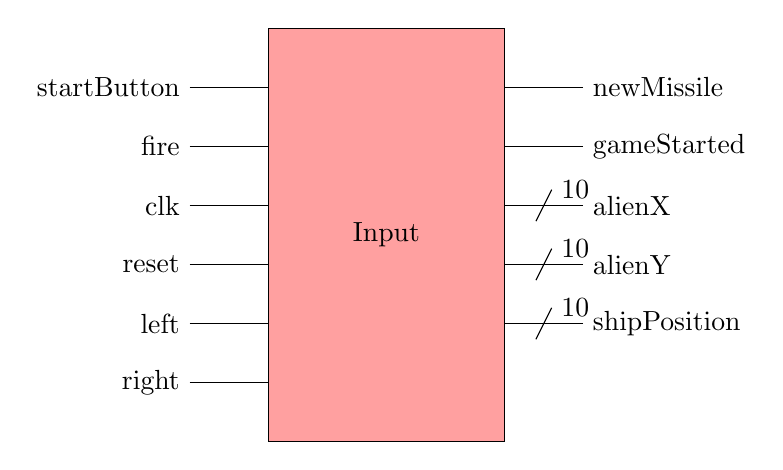
\begin{tikzpicture}
  \draw[fill=blockColor] (0,0) rectangle node{Input}(3,-5.25);
  % Inputs
  \draw (-1,-.75) node[left]{startButton} -- (0,-.75);
  \draw (-1,-1.5) node[left]{fire}-- (0,-1.5);
  \draw (-1,-2.25) node[left]{clk}-- (0,-2.25);
  \draw (-1,-3) node[left]{reset}-- (0,-3);
  \draw (-1,-3.75) node[left]{left}-- (0,-3.75);
  \draw (-1,-4.5) node[left]{right}-- (0,-4.5);
  % Outputs
  \draw (4,-.75) node[right]{newMissile}-- (3,-.75);
  \draw (4,-1.5) node[right]{gameStarted}-- (3,-1.5);
  \draw (4,-2.25) node[right]{alienX}-- (3,-2.25);
  \draw (3.6,-2.05) node[right]{10} -- (3.4, -2.45);
  \draw (4,-3) node[right]{alienY}-- (3,-3);
  \draw (3.6,-2.8) node[right]{10} -- (3.4, -3.2);
  \draw (4,-3.75) node[right]{shipPosition}-- (3,-3.75);
  \draw (3.6,-3.55) node[right]{10} -- (3.4, -3.95);
\end{tikzpicture}
\caption{Schéma bloc}
\label{inputBloc}
\end{wrapfigure}

blabla

\clearpage

\section{rocketManager}
\label{sec:rocketmanager}

\begin{wrapfigure}{r}{.6\textwidth}
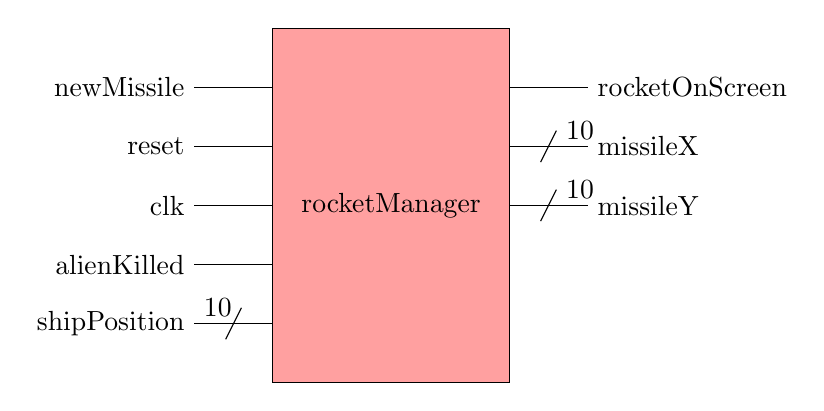
\begin{tikzpicture}
  \draw[fill=blockColor] (0,0) rectangle node{rocketManager}(3,-4.5);
  % Inputs
  \draw (-1,-.75) node[left]{newMissile}-- (0,-.75);
  \draw (-1,-1.5) node[left]{reset}-- (0,-1.5);
  \draw (-1,-2.25) node[left]{clk}-- (0,-2.25);
  \draw (-1,-3) node[left]{alienKilled}-- (0,-3);
  \draw (-1,-3.75) node[left]{shipPosition}-- (0,-3.75);
  \draw (-.4,-3.55) node[left]{10} -- (-.6, -3.95);
  % Outputs
  \draw (4,-.75) node[right]{rocketOnScreen}-- (3,-.75);
  \draw (4,-1.5) node[right]{missileX}-- (3,-1.5);
  \draw (3.6,-1.3) node[right]{10} -- (3.4, -1.7);
  \draw (4,-2.25) node[right]{missileY}-- (3,-2.25);
  \draw (3.6,-2.05) node[right]{10} -- (3.4, -2.45);
\end{tikzpicture}
\caption{Schéma bloc}
\label{rocketManagerBloc}
\end{wrapfigure}

\emph{rocketManager} 

\clearpage

\section{VGA Intenal}
\label{sec:vgainternal}


\begin{wrapfigure}[13]{r}{.55\textwidth}
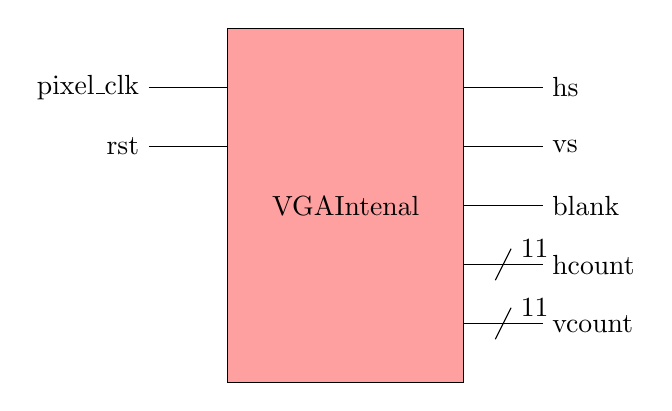
\begin{tikzpicture}
  \draw[fill=blockColor] (0,0) rectangle node{VGAIntenal}(3,-4.5);
  % Inputs
  \draw (-1,-.75) node[left]{pixel\_clk} -- (0,-.75);
  \draw (-1,-1.5) node[left]{rst}-- (0,-1.5);
  % Outputs
  \draw (4,-.75) node[right]{hs}-- (3,-.75);
  \draw (4,-1.5) node[right]{vs}-- (3,-1.5);
  \draw (4,-2.25) node[right]{blank}-- (3,-2.25);
  \draw (4,-3) node[right]{hcount}-- (3,-3);
  \draw (3.6,-2.8) node[right]{11} -- (3.4, -3.2);
  \draw (4,-3.75) node[right]{vcount}-- (3,-3.75);
  \draw (3.6,-3.55) node[right]{11} -- (3.4, -3.95);
\end{tikzpicture}
\caption{Schéma bloc}
\label{vgaInternalBloc}
\end{wrapfigure}

Une interface VGA fonctionne selon les trois composantes RGB ainsi qu’une
synchronisation horizontale et verticale. Les signaux RGB décrivent
la couleur des pixels composant l’image selon un balayage effectué de gauche à
droite, en ligne de haut en bas. L’écran recevant ce flux RGB est capable de
savoir à quel pixel il correspond selon l’instant $t$ auquel il lit ses données
dans le balayage. Néanmoins, ce n’est pas l’écran qui est chargé de sauter
automatiquement à la ligne suivante lorsque chaque pixel de la ligne actuel a
été traité. C’est ce à quoi sert le signal \emph{HS}, alors que \emph{VS} indique un retour à
la première ligne.

\infoInfo{Retour à la ligne}{Afin d’informer le monitor que le
balayage est arrivé à la fin d’une ligne et que le prochain pixel sera le premier de
la ligne suivante, le signal HS produit une impulsion
de synchronisation. De même, lorsque le balayage est
arrivé à la fin de la dernière ligne (et donc que toute
une image a été transmise), le signal VS produit une impulsion pour indiquer un
retour à la première ligne (et donc la transmission d’une nouvelle image).}

Lorsque le balayage se trouve en dehors de l'écran, le signal \emph{blank} prend
comme valeur 0 afin d'indiquer au bloc \emph{Display} de mettre les composantes
de sorties RGB à 0. Ce comportement est définit dans la norme VGA et résulte
dans une erreur d'affichage ``Index out of bound'' s'il n'est pas respecté.

\subsection{Entrées \& Sorties}
\label{subsec:Entrées_Sorties_dmc}

\begin{descr}
  \itemColor{pixel\_clk} Horloge 40MHz, active sur front montant.
  \itemColor{rst} Reset du circuit, actif à l'état haut.
  \itemColor{hs} Impulsion de synchronisation horizontale. Indique par une pulse
  à l'état haut un retour à la ligne du balayage de l'écran.
  \itemColor{vs} Impulsion de synchronisation verticale. Indique par une pulse à
  l'état haut un retour du balayage à la première ligne de l'écran.
  \itemColor{blank} Si 1, le balayage est en dehors de l'écran et les
  composantes RGB, c'est-à-dire les sorties \emph{red}, \emph{blue} et
  \emph{green} doivent être null.
  \itemColor{hcount} Coordonnée $X$ du balayage.
  \itemColor{vcount} Coordonnée $Y$ du balayage.
\end{descr}
\clearpage

\section{Top Module}
\label{sec:topmodule}

\begin{wrapfigure}{r}{.6\textwidth}
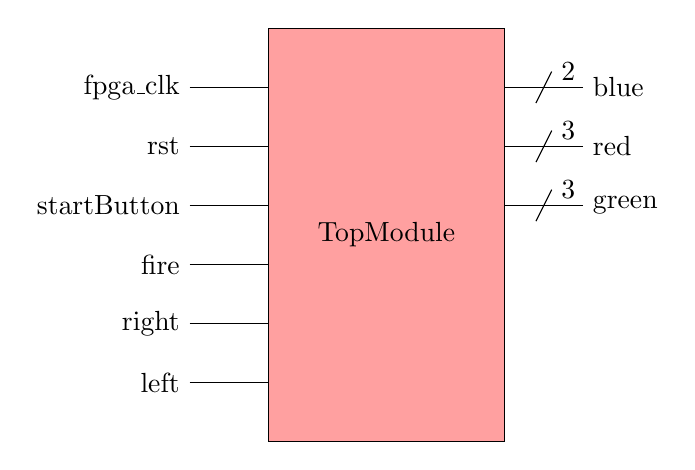
\begin{tikzpicture}
  \draw[fill=blockColor] (0,0) rectangle node{TopModule}(3,-5.25);
  % Inputs
  \draw (-1,-.75) node[left]{fpga\_clk}-- (0,-.75);
  \draw (-1,-1.5) node[left]{rst}-- (0,-1.5);
  \draw (-1,-2.25) node[left]{startButton}-- (0,-2.25);
  \draw (-1,-3) node[left]{fire}-- (0,-3);
  \draw (-1,-3.75) node[left]{right}-- (0,-3.75);
  \draw (-1,-4.5) node[left]{left}-- (0,-4.5);
  % Outputs
  \draw (4,-.75) node[right]{blue}-- (3,-.75);
  \draw (3.6,-.55) node[right]{2} -- (3.4, -.95);
  \draw (4,-1.5) node[right]{red}-- (3,-1.5);
  \draw (3.6,-1.3) node[right]{3} -- (3.4, -1.7);
  \draw (4,-2.25) node[right]{green}-- (3,-2.25);
  \draw (3.6,-2.05) node[right]{3} -- (3.4, -2.45);
\end{tikzpicture}
\caption{Schéma bloc}
\label{topModuleBloc}
\end{wrapfigure}

blabla

\clearpage

\section{Package}
\label{sec:package}

\asymmetricalPage
\chapter{Annexes}

\symmetricalPage

\section{Convertion d'image}
\label{sec:convertPicture}

Le bloc \emph{Display} affiche des données à l'écran en affectant une valeur au
trois signaux \emph{red}, \emph{green} et \emph{blue}. Les deux premiers sont
contenues sur trois bits, alors que le dernier est uniquement sur deux. Celà
signifie que le jeux de couleurs à disposition vaut:
\begin{align*}
  n_{colors} &= 2^{8}\\
             &= 256
\end{align*}

Une couleur est ainsi affectée à chaque pixel, en commançant par celui en haut à
gauche de l'écran, puis celui à sa droite et ainsi de suite jusqu'à arriver à la
droite de l'écran et commencer la ligne suivante. Il apparait alors que puis
afficher une image, il faut extraire le code couleur de chaqu'un de ses pixels,
puis les stocker d'une des deux façon suivantes:\vspace{.1in}
\begin{items}
\item Dans une RAM ou une ROM, celà implique de convertir l'image en un fichier
  \emph{COE} de la forme suivante:
  \begin{lstlisting}[frame=single, basicstyle=\scriptsize, backgroundcolor=\color{backcolor}]
memory_initialization_radix=16;
memory_initialization_vector=
43,
26,
2,
6e,
6e,
4a,
d9,
b6,
6e,
dd,
b5,
6a,
dd,
b6,
6a;
\end{lstlisting}
\emph{memory\_initialization\_radix=16;} indique les valeurs sont stockées en
hexadecimale. Il est possible de le faire en binaire ou en decimal.
\item Dans un tableau 2D:
  \begin{lstlisting}[style=vhdl]
type memoryPicture is array(0 to 4, 0 to 2) of integer;
constant picture : memoryPicture:=(
(16#43#,16#26#,16#2#),
(16#6e#,16#6e#,16#4a#),
(16#d9#,16#b6#,16#6e#),
(16#dd#,16#b5#,16#6a#),
(16#dd#,16#b6#,16#6a#));
  \end{lstlisting}
\end{items}

Avec un COE, chaque valeur est stocké à la suite. En utilisant un tableau VHDL,
il est possible de stocker en deux dimensions les valeurs pour avoir une
représentation identique à celle de l'écran. La forme \emph{16\#<value>\#} indique
en VHDL que le nombre est sous forme hexadecimale et peut être directement
assigné à un signal de type sdl\_logic\_vector.

Afin de rapidement convertir des images en fichier COE ou en tableau 2D VHDL,
nous avons écris un script Matlab. Le détail de son fonctionnement est inclus
dans les commentaires du code.

\infoInfo{Format des images}{Seul les images au format ``JPG'' sont supportés
  par le script.}

\clearpage

\subsection{Script Matlab - Convertion en fichier COE}
\label{subsec:Script1}
\vspace{.1in}
\lstinputlisting[style=matlab]{matlab/picturesToCOE.m}
\clearpage

\subsection{Script Matlab - Convertion en tableau VHDL}
\label{subsec:Script2}
\vspace{.1in}
\lstinputlisting[style=matlab]{matlab/picturesToFPGA.m}


\end{document}